\documentclass[a4paper]{article}

%% Language and font encodings
\usepackage[spanish]{babel}
\usepackage[utf8x]{inputenc}
\usepackage[T1]{fontenc}
\usepackage{listings}
\spanishdecimal{.}


%% Sets page size and margins
\usepackage[a4paper,top=3cm,bottom=2cm,left=3cm,right=3cm,marginparwidth=1.75cm]{geometry}

%% Useful packages
\usepackage{amsmath}
\usepackage{graphicx}
\usepackage[colorinlistoftodos]{todonotes}
\usepackage[colorlinks=true, allcolors=blue]{hyperref}

\title{Práctica 8: modelo de urnas}
\begin{document}
\maketitle

\section{Introducci\'on}
En esta práctica trabajaremos algo llamado fenómenos de coalescencia y fragmentación, supongamos que tenemos alguna solución y deseamos filtrar una determinada partícula, una de las características más relevantes de dicha partícula es su tamaño. Se cuenta con una red que solo captura las partículas del tamaño que se especifique, es por esto que como parte del contexto de la prueba se desea tener un tamaño determinado de partículas para su mejor manejo. 

Se cuenta con códigos iniciales los cuales se encuentran el la siguiente \href{http://elisa.dyndns-web.com/teaching/comp/par/p8.html}{página web}. Los primero códigos nos ayudan a saber si las partículas permanecen en una distribución normal, después se le asigna a las partículas una probabilidad de fractura según su tamaño, se espera que si es una partícula grande, por encima de la media tiene una probabilidad mayor de ser fracturada, en cambio, si es una partícula pequeña se espera que se pueda unir a otra partícula pequeña, para que así se puedan acercar estas partículas al tamaño deseado, a dichas partículas de volumen se les llamará cúmulos. El objetivo de la práctica es saber si se ahorra tiempo de ejecución cuando se paraleliza el código, es por eso que se toman en cuenta tanto el código original, solo con las modificaciones que miden los tiempos, así como el código que se paralelizó.

\section{Par\'ametros de trabajo}
Las pruebas se corrieron en una iMac con procesador 3.1 Ghz, Intel Core i7 con 16 GB de memoria y 1600 Mhz y con ocho núcleos. Se contemplarán los requerimientos del reto uno, así la variable \textit{n} representa la cantidad total de partículas y estará en relación con \textit{k}, que es la cantidad de cúmulos existentes, de esta forma existirán $30$ veces la cantidad de cúmulos. Los cúmulos se variaron de la siguiente manera $k\in\{10000,20000,35000,50000\}$, para cada uno de los cambios de cúmulos se realizaron 100 repeticiones, así mismo se corrieron tanto el código secuencial como el paralelizado en la misma máquina.

\section{Modificaciones del código}
Del código original solo se le agregó un ciclo \texttt{for} el cual contiene las variaciones de los parámetros, así como el contador de tiempo que necesita para cada repetición, también fue necesario agregar un \textit{data.frame} con el fin de poder guardar todos los tiempos de ejecución para su posterior análisis.

\begin{lstlisting}[frame=single]
v <- c(10000,20000,35000,50000)
veces <- length(v)
tiempsec <- data.frame()

for(e in 1:veces){
library(testit) # para pruebas, recuerda instalar antes de usar
k <- v[e]
n <- k*30
...
for (paso in 1:duracion) {
a <- Sys.time()
...
 b <- Sys.time()
 ti <- c(a,b)
 tie <- diff(ti,units="secs")
 tiempsec <- rbind(tiempsec,c(k,tie))
 } }
\end{lstlisting}

Estas mismas modificaciones se pueden encontrar en el código de paralización, de igual forma se incluyen los comandos necesarios para el uso de los núcleos, incluyendo variables que pudiera usar, y de igual forma se llama la librería \texttt{parallel}.

\begin{lstlisting}[frame=single]
library(parallel)
cluster <- makeCluster(detectCores() - 1)
clusterExport(cluster, "faserotura")
clusterExport(cluster, "romperse")
clusterExport(cluster, "rotura")
...
c <- Sys.time()

assert(sum(cumulos) == n)
cumulos <- integer()
clusterExport(cluster, "freq")
cumulos <- parSapply(cluster, 1:dim(freq)[1], faserotura)
cumulos <- unlist(cumulos)
...
\end{lstlisting}

La última modificación que se realizó fue que los valores de los datos para ambas ejecuciones se mandaron escribir a un archivo con formato \texttt{csv} con el fin de poderlo recuperar para el análisis y la generación de gráficos.
\section{Resultados}
Los tiempos de ejecución para cada uno de los códigos los podemos ver representados en las figuras \ref{fig:Vnoparalelo} y \ref{fig:Vparalelo}.

\begin{figure}[h]
\centering
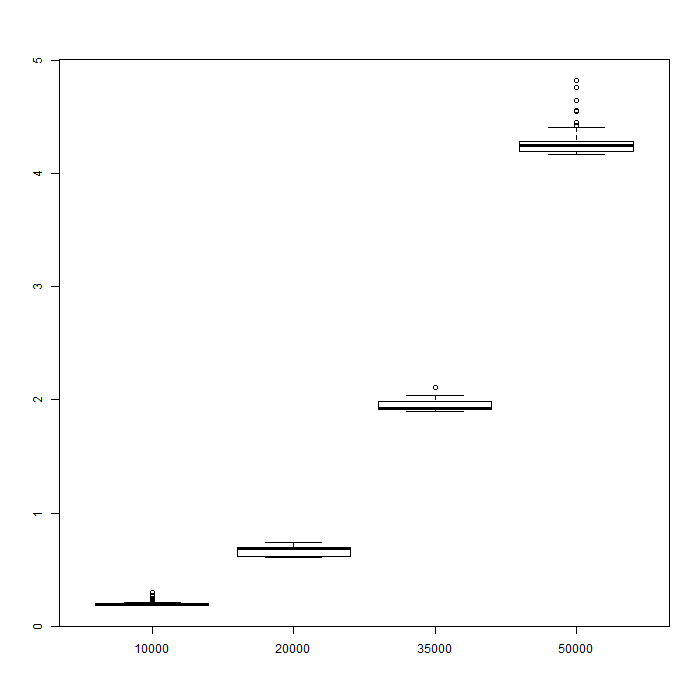
\includegraphics[width=0.7\linewidth]{Vnoparalelo}
\caption{Se presentan los tiempos de ejecución por corrida agrupados por la cantidad de cúmulos en cada uno para la ejecución sin paralelización.}
\label{fig:Vnoparalelo}
\end{figure}

\begin{figure}[h]
\centering
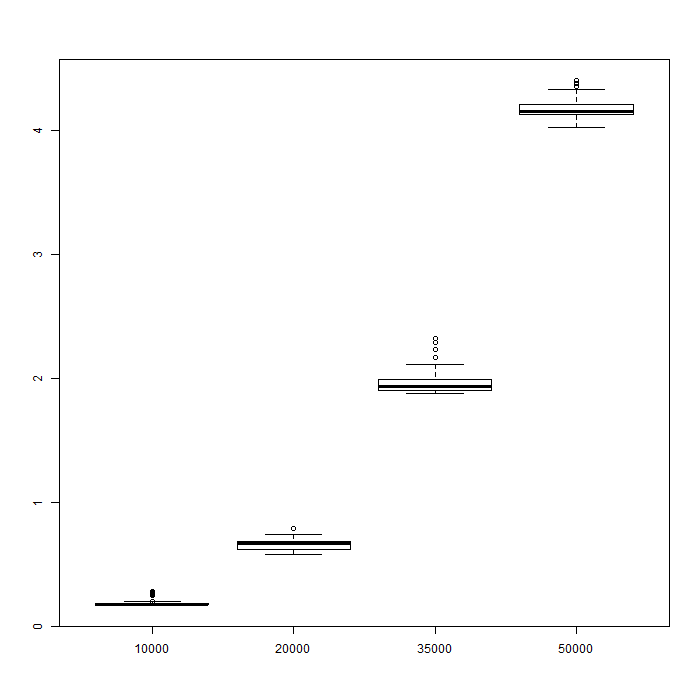
\includegraphics[width=0.7\linewidth]{Vparalelo}
\caption{Se presentan los tiempos de ejecución por corrida agrupados por la cantidad de cúmulos en cada uno para la ejecución paralelizada.}
\label{fig:Vparalelo}
\end{figure}

Para ambos casos es notorio el incremento de los tiempos al momento de aumentar el número de partículas, desafortunadamente de esto aún no se pudo inferir algo.

\subsection{Análisis estadístico}
En la figura \ref{fig:ambos} se presenta de modo gráfico los tiempos de ambas pruebas, si se observa con detalle es muy difícil conjeturar por los gráficos que modo de corrida te ahorra tiempo en la ejecución.

\begin{figure}[h]
	\centering
	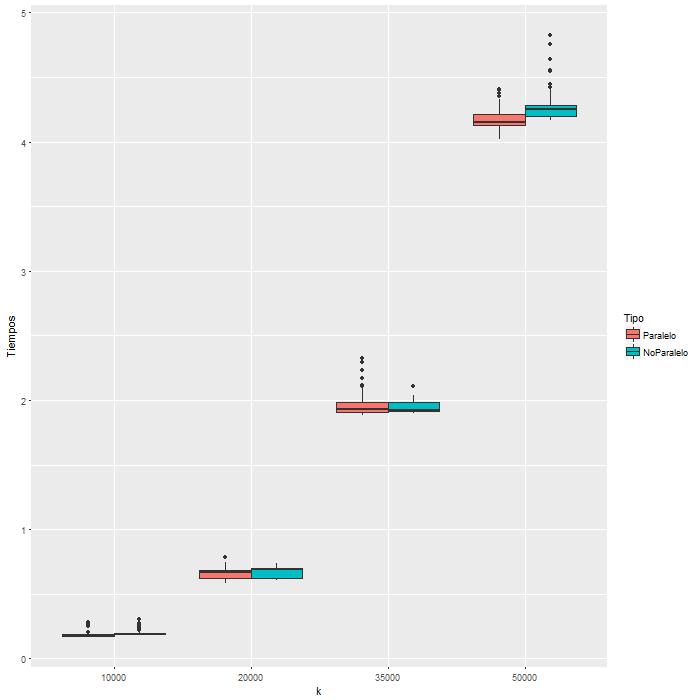
\includegraphics[width=0.7\linewidth]{ambos}
	\caption{Tiempos de ejecución en segundos para ambos códigos}
	\label{fig:ambos}
\end{figure}

Es por esto que es necesario el análisis estadístico, se realizó primero una prueba de normalidad para saber si era posible utilizar alguna prueba para-métrica con las medias de los tiempos, y se descubrió que no era posible, por tanto fue necesario recurrir a una prueba no para-métrica como lo es el test de Wilcox, del cual obtuvimos los siguientes resultados.

\begin{lstlisting}[frame=single]
> wilcox.test(ambos$Tiempos[ambos$Tipo=="Paralelo"],
ambos$Tiempos[ambos$Tipo=="NoParalelo"] )

Wilcoxon rank sum test with continuity correction

data:  ambos$Tiempos[ambos$Tipo == "Paralelo"] and 
ambos$Tiempos[ambos$Tipo == "NoParalelo"]
W = 71920, p-value = 0.01342
alternative hypothesis: true location shift is not equal to 0
\end{lstlisting}

Lo relevante de los datos anteriores es el $p$-value, el cual nos indica que si existe una diferencia significativa entre las medias de los tiempos, se procede a observar que media es mayor y por tanto que código nos ahorra tiempos de ejecución.

\begin{lstlisting}[frame=single]
> median(ambos$Tiempos[ambos$Tipo=="Paralelo"])
[1] 1.335076
> median(ambos$Tiempos[ambos$Tipo=="NoParalelo"])
[1] 1.319076
> 
\end{lstlisting}

De esto podemos inferir que de modo general los tiempos sin importar el tamaño de la muestra son menores con el código no paralelizado. 

\section{Conclusiones}
Es necesario comprobar que cualquier cosa que lleguemos a paralelizar valga realmente el esfuerzo de paralelizarlo, es decir, podremos encontrar implementaciones como la realizada en esta prueba que no sea lo suficientemente compleja como para hacerlo. Este es un claro ejemplo que los problemas sencillos o con cantidad de variables no tan grandes no es necesario paralelizarlos, ya que le exiges más a la maquina de lo que se necesita de modo secuencial.

\end{document}